\documentclass{article}
\usepackage[utf8]{inputenc}
\usepackage{graphicx}
\usepackage{geometry}
\geometry{a4paper, margin=1in}
\title{Student Performance Dataset - Descriptive and Predictive Analysis}
\author{Group Assignment}
\date{\today}
\begin{document}
\maketitle
\section{Hadoop and Hive Environment Startup}
The Hadoop Distributed File System (HDFS) and YARN resource manager were successfully started in the local cluster environment. Data was uploaded from the local file system into HDFS, and the Hive Metastore service was initialized on port 9083 to enable Hive queries via Beeline.
\begin{figure}[h!]
\centering
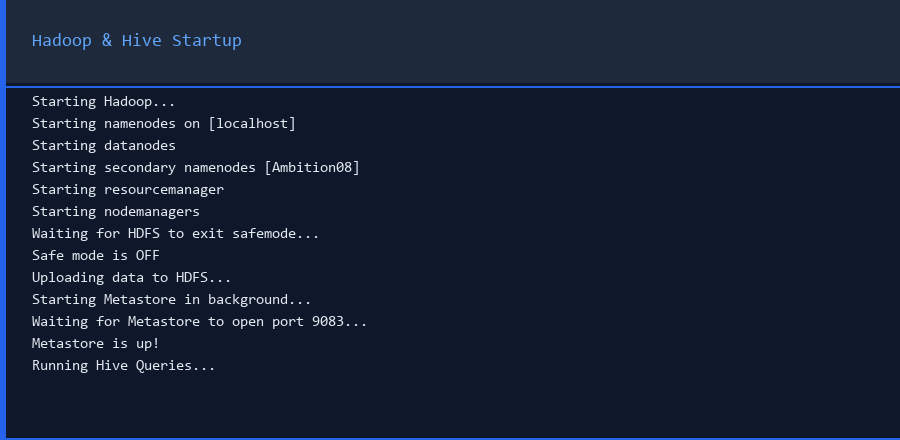
\includegraphics[width=0.9\textwidth]{images/00_hadoop_startup.png}
\caption{Hadoop Cluster and Metastore Startup Process}
\end{figure}
\clearpage
\section{Task 1: Total Students by Department}
\begin{figure}[h!]
\centering
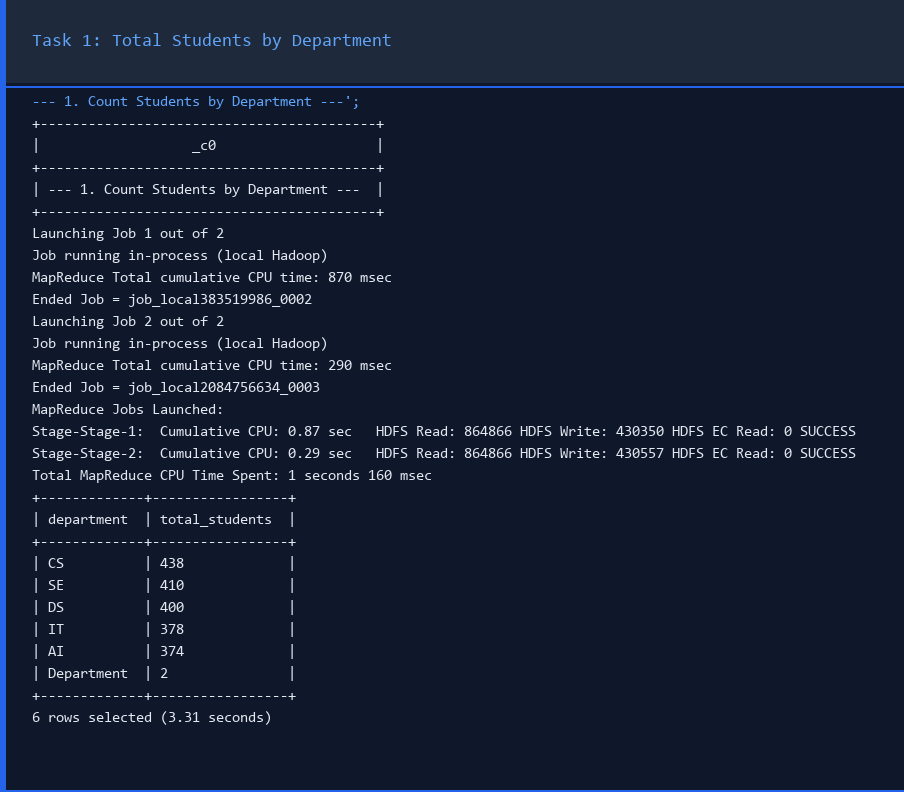
\includegraphics[width=0.9\textwidth]{images/01_student_count_by_dept.png}
\caption{Task 1: Total Students by Department}
\end{figure}
\clearpage
\section{Task 2: Average GPA by Department}
\begin{figure}[h!]
\centering
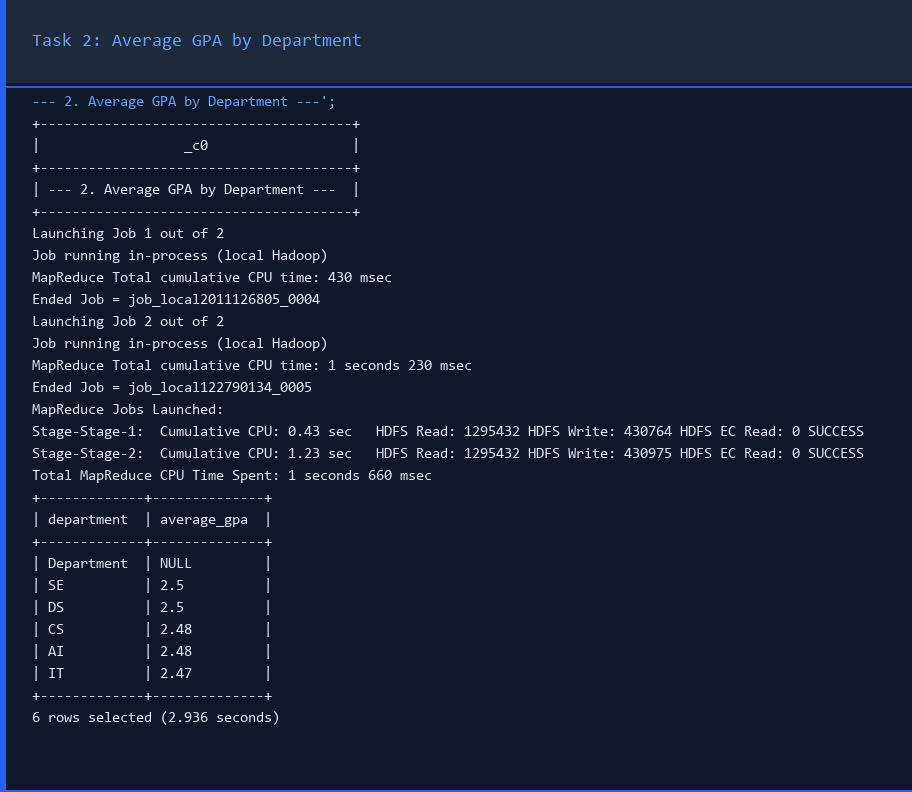
\includegraphics[width=0.9\textwidth]{images/02_average_gpa_dept.png}
\caption{Task 2: Average GPA by Department}
\end{figure}
\clearpage
\section{Task 3: Students with Attendance Below 60%}
\begin{figure}[h!]
\centering
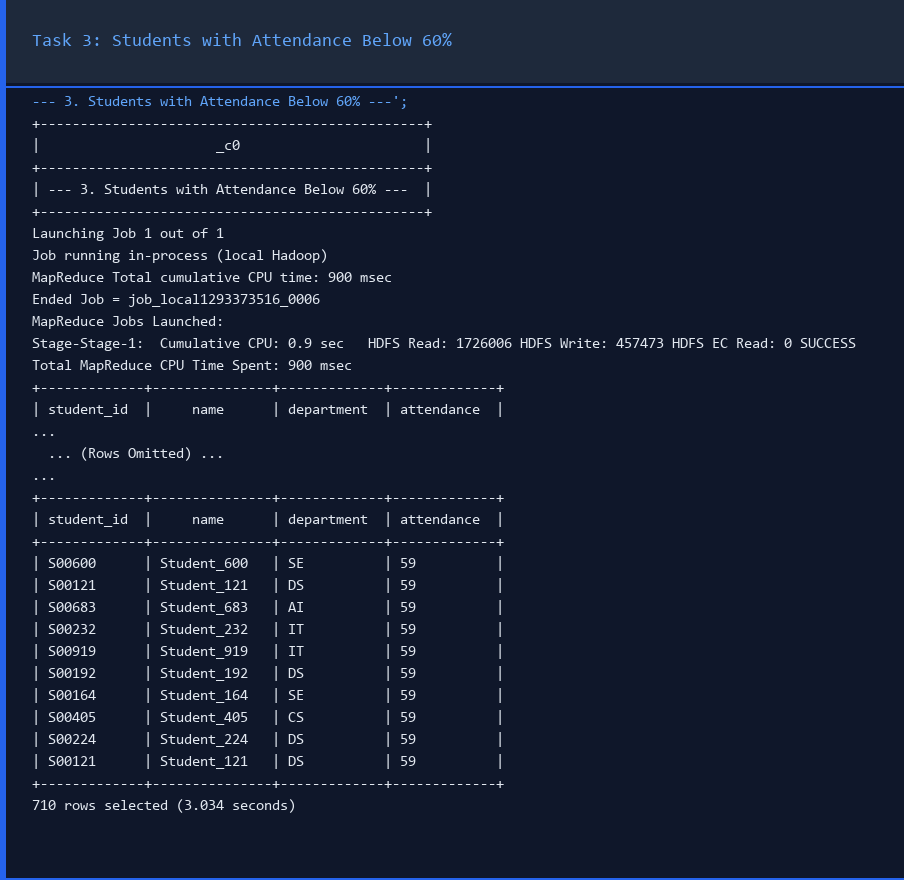
\includegraphics[width=0.9\textwidth]{images/03_attendance_below_60.png}
\caption{Task 3: Students with Attendance Below 60%}
\end{figure}
\clearpage
\section{Task 4: Placement Rate by Program}
\begin{figure}[h!]
\centering
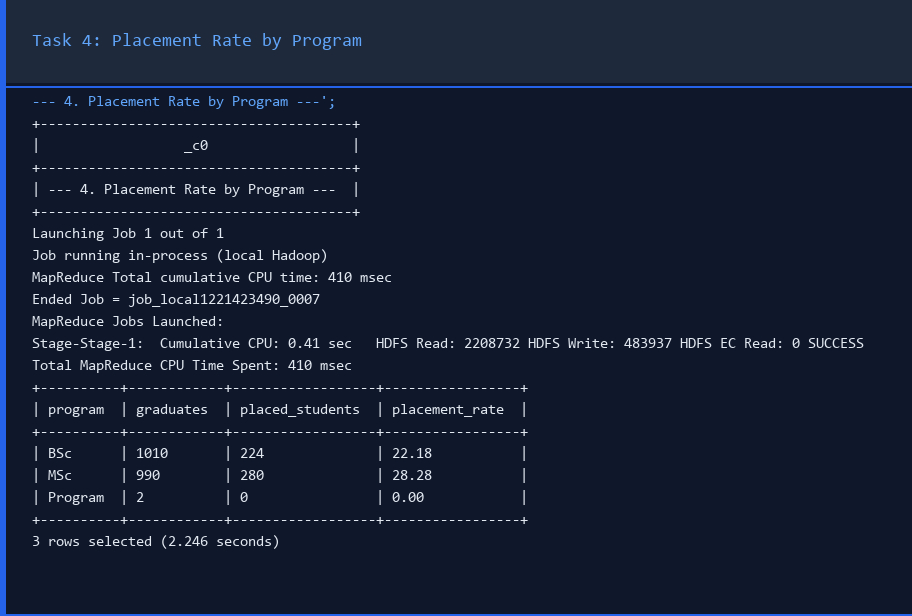
\includegraphics[width=0.9\textwidth]{images/04_placement_rate.png}
\caption{Task 4: Placement Rate by Program}
\end{figure}
\clearpage
\section{Task 5: Ranking Students Within Departments}
\begin{figure}[h!]
\centering
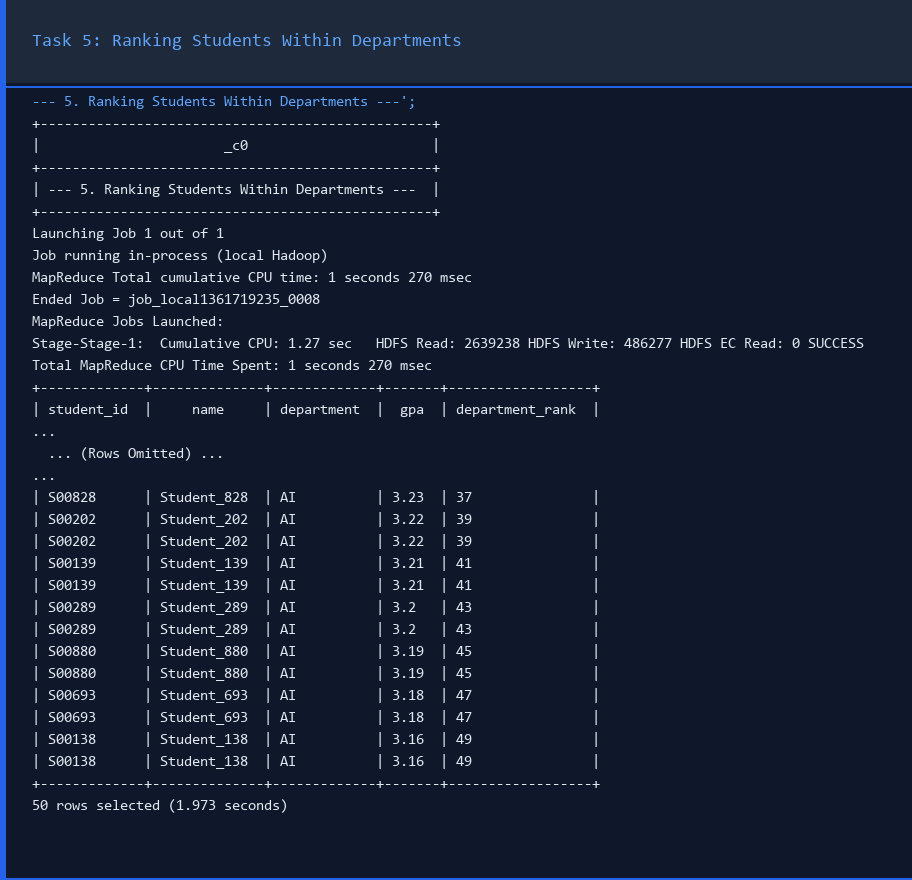
\includegraphics[width=0.9\textwidth]{images/05_ranking_students.png}
\caption{Task 5: Ranking Students Within Departments}
\end{figure}
\clearpage
\end{document}